\section{\textit{Sea Surface Height Edition}}\label{sec:interp_challenge}

Sea surface height (SSH) is one of the most critical, observable quantities when determining the ocean state. 
It is widely used to study ocean dynamics and the adverse impact on global climate and human activities~\cite{SSHMESOSCALE}. 
SSH enables us to track phenomena such as currents and eddies~\cite{SSHMESOSCALE,SSHMESOSCALE2,SSHMESOSCALE3}, which leads to a better quantification of the transport of energy, heat, and salt. 
In addition, SSH helps us quantify sea level rise at regional and global scales~\cite{SSHSEALEVEL,OCEANSEALEVEL}, which is used for operational monitoring of the marine environment~\cite{SSHOPERATIONAL}. 
Furthermore, SSH characterization provides a plethora of data products that downstream tasks can use for many other applications~\cite{SSH3DCIRCULATION, 3DQGOC}.
%
Due to the irregular sampling delivered by satellite altimeter, state-of-the-art operational methods using optimal interpolation schemes~\cite{DUACS, MIOST} or model-driven data assimilation~\cite{DINEOF, DINEOF2, ANALOGDA, ANALOGDA2} fail to fully retrieve SSH dynamics at fine scales below 100-200km on a global or regional scale, so improving the space-time resolution of SSH fields has been a critical challenge in ocean science. 
Beyond some technological developments~\cite{SWOT}, recent studies support the critical role of ML-based schemes in overcoming the current limitations of the operational systems~\cite{4DVARNETSWOT, BFNQG, SSHInterpAttention} .  
%
The rest of this section gives an overview of the general problem definition for SSH interpolation, followed by a brief ontology for ML approaches to address the problem. 
We also give an overview of some experimental designs and datasets with a demonstration of metrics and plots generated by the \texttt{OceanBench} platform. 

% \subsection{Problem general description}

% \textcolor{red}{[Wouldn't it be good to have a slightly more palatable problem description before the mathematical formalism of the next subsection ? ]}


% \textcolor{red}{[Here's an example of one of Florian's paper intro, just to see if this kind of tone fits.]}





\subsection{Problem Definition}\label{sec:prob_definition}
 % \textcolor{red}{or Mathematical formalism}

We are dealing with satellite observations, so we are interested in the domain across the Earth's surface. 
Let us define the Earth's domain by some spatial coordinates, $\mathbf{x} = [\text{Longitude},\text{Latitude}]^\top \in\mathbb{R}^{D_s}$, and temporal coordinates, $t=[\text{Time}]\in\mathbb{R}^+$, where $D_s$ is the dimensionality of the coordinate vector.  
We can define some spatial (sub-)domain, $\Omega\subseteq\mathbb{R}^{D_s}$, and a temporal (sub-)domain, $\mathcal{T}\subseteq\mathbb{R}^+$. 
This domain could be the entire globe for 10 years or a small region within the North Atlantic for 1 year.
%
%
\begin{align}  \label{eq:spatiotemporal_coords}
    \text{Spatial Coordinates}: && \mathbf{x} &\in \Omega \subseteq \mathbb{R}^{D_s}\\ 
    \text{Temporal Coordinates}: && t &\in \mathcal{T} \subseteq \mathbb{R}^+.
\end{align}
%
%
In this case $D_s=2$ because we only have a two coordinates, however we can do some coordinate transformations like spherical to Cartesian. Likewise, we can do some coordinate transformation for the temporal coordinates like cyclic transformations or sinusoidal embeddings~\cite{ATTENTION}. We have two fields of interest from these spatiotemporal coordinates: the state and the observations.
%
%
\begin{align} \label{eq:state_obs}
    \text{State}: && \boldsymbol{u}(\mathbf{x},t) &: \Omega\times\mathcal{T}\rightarrow\mathbb{R}^{D_u} \\
    \text{Observations}: && \boldsymbol{y}_{obs}(\mathbf{x},t) &: \Omega\times\mathcal{T}\rightarrow\mathbb{R}^{D_{obs}}
\end{align}
%
%
The state domain, $u\in\mathcal{U}$, is a scalar or vector-valued field of size $D_u$ which is typically the quantity of interest and the observation domain, $y_{obs}\in\mathcal{Y}_{obs}$, is the observable quantity which is also a scalar or vector-valued field of size $D_{obs}$. Now, we make the assumption that we have an operator $\mathcal{H}$ that transforms the field from the state space, $\boldsymbol{u}$, to the observation space, $\boldsymbol{y}_{obs}$.
%
%
\begin{align} \label{eq:prob_definition}
    \boldsymbol{y}_{obs}(\mathbf{x},t) = \mathcal{H}\left(\boldsymbol{u}(\mathbf{x},t), t, \boldsymbol{\varepsilon}, \boldsymbol{\mu}\right) 
\end{align}
%
%
This equation is the continuous function defined over the entire spatiotemporal domain.  
The operator, $\mathcal{H}(\cdot)$, is flexible and problem dependent.
For example, in a some discretized setting there are 0's wherever there are no observations, and 1's wherever there are observations, and in other discretized settings it takes a weighted average of the neighboring pixels.
We also include a generic noise function, $\boldsymbol{\varepsilon}(\mathbf{x},t)$.
This could stem from a distribution, it could stationary noise operator, $\boldsymbol{\varepsilon}(\mathbf{x})$, or it could be constant in space but vary with Time, $\boldsymbol{\varepsilon}(t)$. 
We also include a control parameter, $\boldsymbol{\mu}$, representing any external factors or latent variables that could connect the state vector to the observation vector, e.g., sea surface temperature.
%
%###########################################################################################
%
% CAN BE FRAMED AS INVERSE PROBLEMS
%
Our quantity of interest is SSH, $\eta$, a scalar-valued field defined everywhere on the domain. In our application, we assume that the SSH we observe from satellite altimeters, $\eta_{obs}$, is the same as the SSH state, except it could be missing for some coordinates due to incomplete coverage from the satellite. So our transformation is defined as follows:
%
\begin{align} \label{eq:ssh_field_continuous}
\boldsymbol{\eta}_{obs}(\mathbf{x},t) &= \mathcal{H}\left(\boldsymbol{\eta}(\mathbf{x},t), t, \boldsymbol{\varepsilon}, \boldsymbol{\mu}\right)
% , \hspace{10mm}
% \mathbf{x} \in \Omega \subseteq \mathbb{R}^{D_s}, \hspace{10mm} 
% t \in \mathcal{T} \subseteq \mathbb{R}^+.
\end{align}
%
In practice, the satellite providers have a reasonable estimation of the amount of structured noise level we can expect from the satellite altimetry data; however, unresolved noise could still be present. 
% Although we do not explicitly specify the control parameter, $\boldsymbol{\mu}$, we leave it into the equation to account for any other state parameters not accounted for in our model. 
Finally, we are interested in finding some model, $\mathcal{M}$, that maps the SSH we observe to the true SSH given by
%
\begin{align} \label{eq:interp_problem}
    \mathcal{M} &: \boldsymbol{\eta}_{obs}(\mathbf{x}, t, \boldsymbol{\mu}) \rightarrow \boldsymbol{\eta}(\mathbf{x},t),
%     , \hspace{10mm}
% \mathbf{x} \in \Omega \subseteq \mathbb{R}^{D_s}, \hspace{10mm} 
% t \in \mathcal{T} \subseteq \mathbb{R}^+.
\end{align}
%
which is essentially an inverse problem that maps the observations to the state.
One could think of it as trying to find the inverse operator, $\mathcal{M}=\mathcal{H}^{-1}$, but this could be some other arbitrary operator.  
%
\subsection{Machine Learning Model Ontology} \label{sec:ml_ontology_mini}

In general, we are interested in finding some parameterized operator, $\mathcal{M}_{\boldsymbol{\theta}}$, that maps the incomplete SSH field to the complete SSH field
%
%
\begin{align} \label{eq:ml_interp_problem}
    \mathcal{M}_{\boldsymbol{\theta}} &: \boldsymbol{\eta}_{obs}(\mathbf{x}, t, \boldsymbol{\mu}) \rightarrow \boldsymbol{\eta}(\mathbf{x},t),
\end{align}
%
whereby we learn the parameters from data.
%
The two main tasks we can define from this problem setup are 1) interpolation and 2) extrapolation.
We define \textit{interpolation} as the case when the boundaries of the inferred state domain lie within a predefined shape for the boundaries of the spatiotemporal observation domain. 
For example, the shape of the spatial domain could be a line, box, or sphere, and the shape of the temporal domain could be a positive real number line.
We define \textit{extrapolation} as the case where the boundaries of the inferred state domain are outside the boundaries of the spatiotemporal observation domain. 
In this case, the inferred state domain could be outside of either domain or both. 
A prevalent specific case of extrapolation is \textit{hindcasting} or \textit{forecasting}, where the inferred state domain lies within the spatial observation domain's boundaries but outside of the temporal observation domain's.
In the rest of this paper, we will look exclusively at the interpolation problem. 
However, we refer the reader to appendix~\ref{sec:other_tasks} for a more detailed look at other subtasks that can arise.

From a ML point of view, we can explore various ways to define the operator in equation~\eqref{eq:interp_problem}. 
We may distinguish three main categories: (i) coordinate-based methods that learn a parameterized continuous function to map the domain coordinates to the scalar values, (ii) the explicit mapping of the state from the observation, (iii) implicit methods defined as the solution of an optimization problem. 
The first category comprises of kriging approaches, which have been used operationally with historical success~\cite{KRIGINGREVIEW,DUACS}. Beyond such covariance-based approaches, recent contributions explore more complex trainable functional models~\cite{GPsBIGDATA}, basis functions~\cite{MIOST}, and neural networks~\cite{NERFSSSH}. 
The second category of schemes bypasses the physical modeling aspect and amortizes the prediction directly using state-of-the-art neural architectures such as UNets and ConvLSTM ~\cite{SSHInterpAttention, SSHInterpConvLSTM, SSHInterpUNet}. 
This category may straightforwardly benefit from available auxiliary observations, including available operational gap-free SST products and other sea surface tracers, to state the interpolation problem as a super-resolution~\cite{SuperResSurvey} or image-to-image translation problem~\cite{IMAGE2IMAGETRANSLATION, IMAGE2IMAGETRANSLATION2}. 
The third category relates to inverse problem formulations and associated deep learning schemes, for example deep unfolding methods and plug-and-play priors~\cite{DEEPUNFOLDING}. 
Interestingly, recent contributions explore novel neural schemes which combine data assimilation formulations~\cite{DAGEOSCIENCE} and learned optimizer strategies~\cite{4DVARNETSWOT,4DVARNETSST}.
We provide a more detailed ontology of methods used for interpolation problems in appendix~\ref{sec:ml_ontology}. 
We consider at least one baseline approach from each category for each data challenge described in section~\ref{sec:data_challenges}. 
While all these methods have pros and cons, we expect OceanBench to lead to new experimental evidence and understanding regarding their applicability to SSH interpolation problems.
 

\subsection{Experimental Design} \label{sec:experimental_design}

The availability of multi-year simulation and observation datasets naturally advocates for the design of synthetic (or twin) experiments, referred to as observing system simulation experiments (OSSE), and of real-world experiments, referred to as observing system experiments (OSE).
We outline these two experimental setups below.

\textbf{Observing System Simulation Experiments (OSSE)}. A staple and groundtruthed experimental setup uses a reference simulation dataset to simulate the conditions we can expect from actual satellite observations. 
This setup allows researchers and operational centers to create a fully-fledged pipeline that mirrors the real-world experimental setting.
An ocean model simulation is deployed over a specified spatial domain and period, and a satellite observation simulator is deployed to simulate satellite observations over the same domain and period. 
This OSSE setup has primarily been considered for performance evaluation, as one can assess a reconstruction performance over the entire space-time domain. It also provides the basis for the implementation of classic supervised learning strategies~\cite{SSHInterpUNet,SSHInterpConvLSTM,SSHInterpAttention}.
The domain expert can vary the experimental conditions depending on the research question. 
For example, one could specify a region based on the expected dynamical regime~\cite{DCOSSEGULFSSH} or add a certain noise level to the observation tracks based on the satellite specifications.
The biggest downside to OSSE experiments is that we train models exclusively with ocean simulations which could produce models that fail to generalize to the actual ocean state. 
Furthermore, the simulations are often quite expensive, which prevents the community from having high spatial resolution over very long periods, which would be essential to capture as many dynamical regimes as possible.


\begin{figure}[t!]
\small
\begin{center}
\setlength{\tabcolsep}{1pt}
\begin{tabular}{ccc}
NADIR Altimetry Tracks & 
SWOT Altimetry Tracks &
Sea Surface Temperature \\
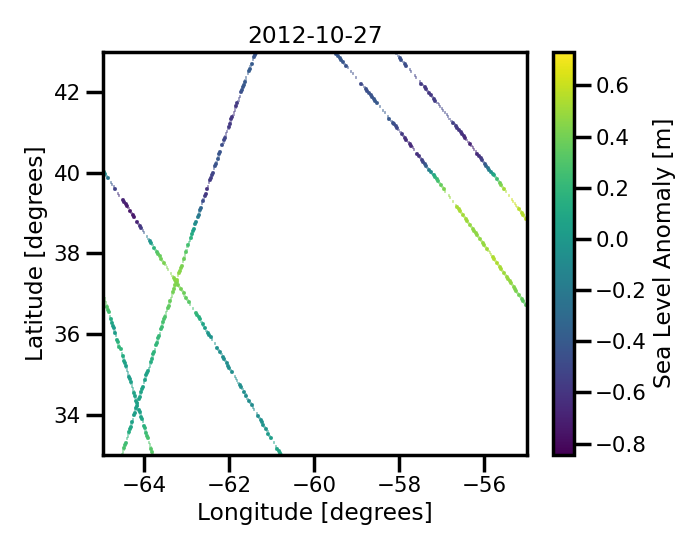
\includegraphics[width=4.25cm,height=3cm]{content/figures/maps/sla/dc20a_ssh_anomaly_nadir4_2012-10-27.png} 
&
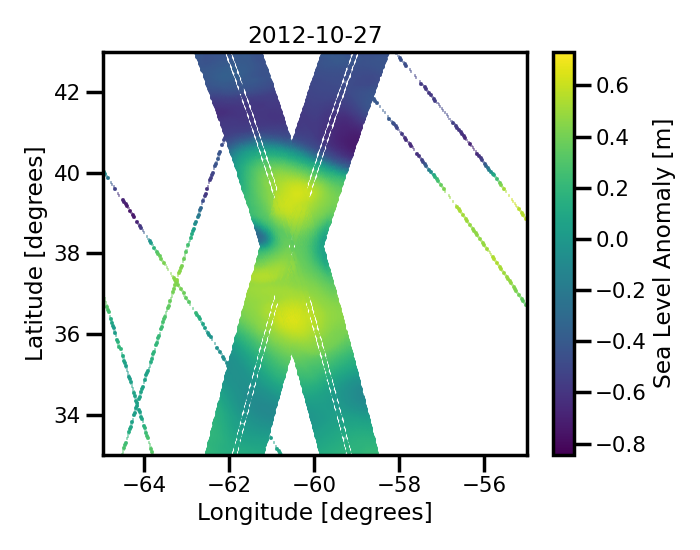
\includegraphics[width=4.25cm,height=3cm]{content/figures/maps/sla/dc20a_ssh_anomaly_swot1nadir5_2012-10-27.png} &
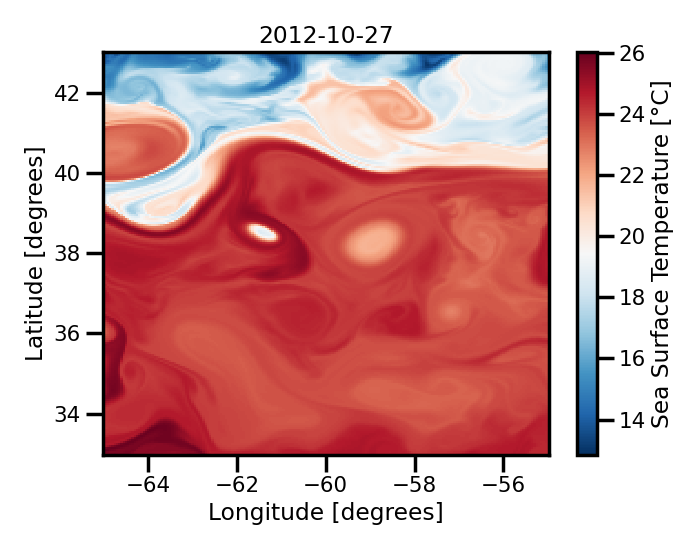
\includegraphics[width=4.25cm,height=3cm]{content/figures/maps/sst/dc20a_nemo_sst.png}
\end{tabular}
\begin{tabular}{cccc}
\hspace{3mm} NEMO Simulation & 
\hspace{3mm} MIOST & 
\hspace{3mm} BFNQG & 
4DVarNet \\
\vspace{-2mm}
%%%%% SEA LEVEL ANOMALY %%%%%%%%
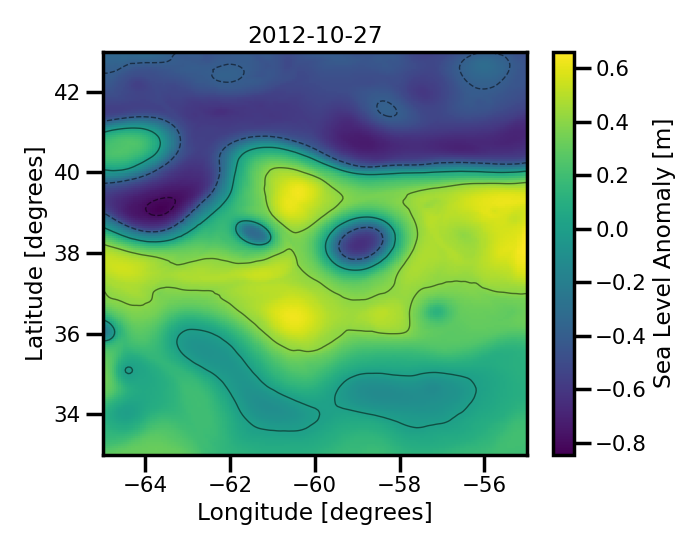
\includegraphics[trim={0 0 42mm 0},clip, width=3.20cm,height=3cm]{content/figures/maps/sla/dc20a_nemo_sla.png} &
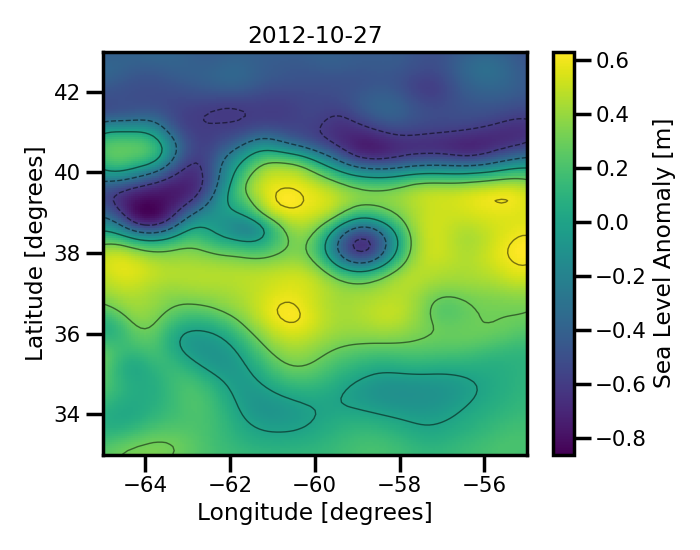
\includegraphics[trim={0 0 42mm 0},clip, width=3.2cm,height=3cm]{content/figures/maps/sla/dc20a_miost_sla.png} &
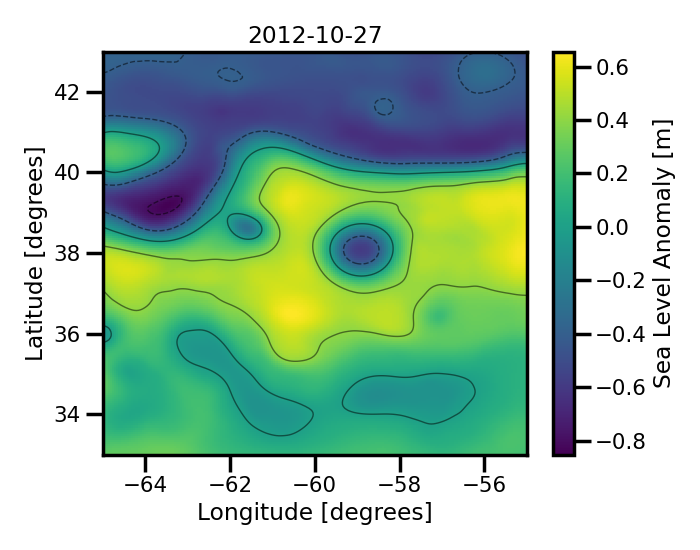
\includegraphics[trim={0 0 42mm 0},clip, width=3.2cm,height=3cm]{content/figures/maps/sla/dc20a_bfnqg_sla.png} &
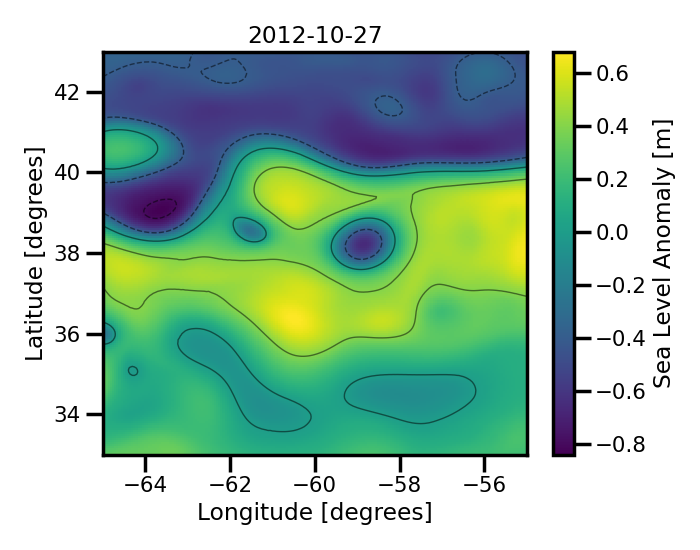
\includegraphics[width=4.0cm,height=3cm]{content/figures/maps/sla/dc20a_4dvarnet_sla.png} \\
\vspace{-2mm}
%%%%% KINETIC ENERGY %%%%%%%%
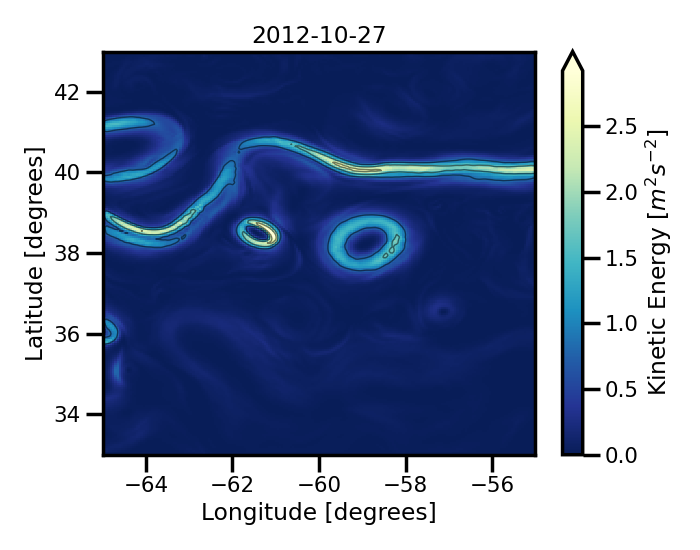
\includegraphics[trim={0 0 42mm 0},clip, width=3.20cm,height=3cm]{content/figures/maps/ke/dc20a/nadir4/dc20a_nemo_ke.png} &
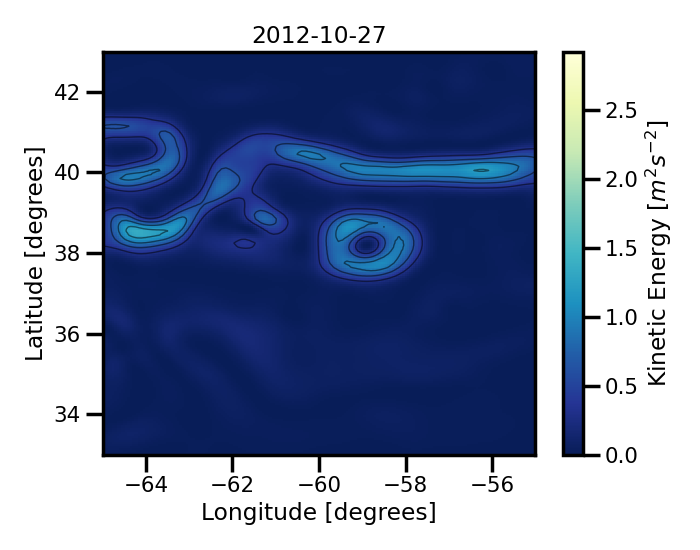
\includegraphics[trim={0 0 42mm 0},clip, width=3.2cm,height=3cm]{content/figures/maps/ke/dc20a/nadir4/dc20a_miost_ke.png} &
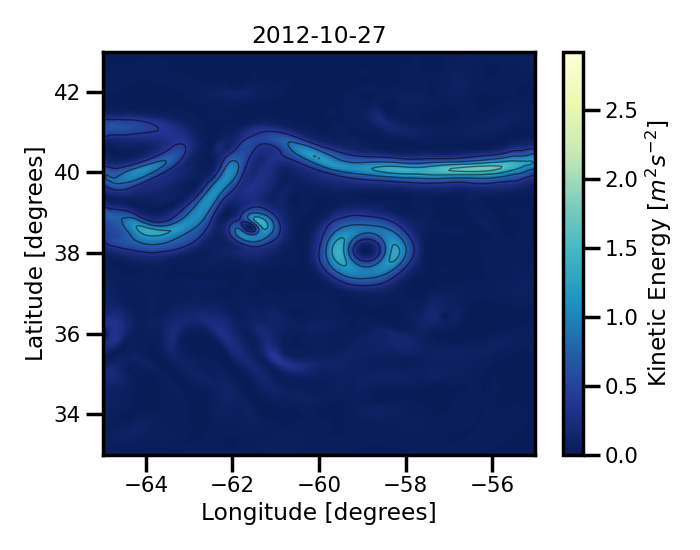
\includegraphics[trim={0 0 42mm 0},clip, width=3.2cm,height=3cm]{content/figures/maps/ke/dc20a/nadir4/dc20a_bfnqg_ke.png} &
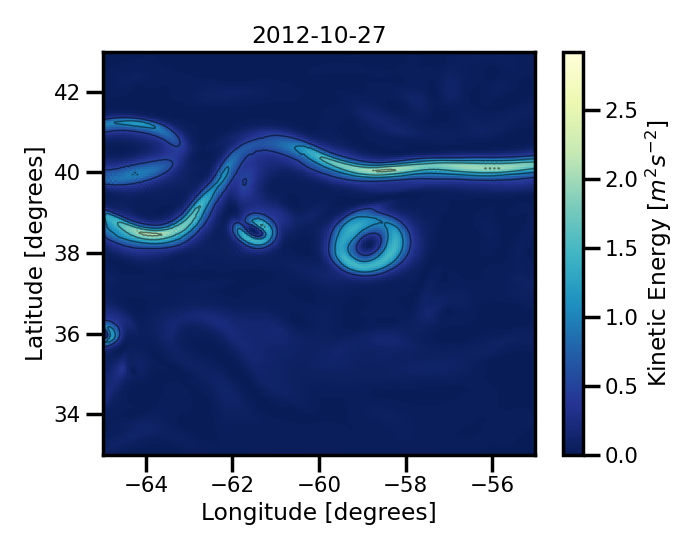
\includegraphics[width=4.0cm,height=3cm]{content/figures/maps/ke/dc20a/nadir4/dc20a_4dvarnet_ke.png}  \\
\vspace{-2mm}
%%%%% RELATIVE VORTICITY %%%%%%%%
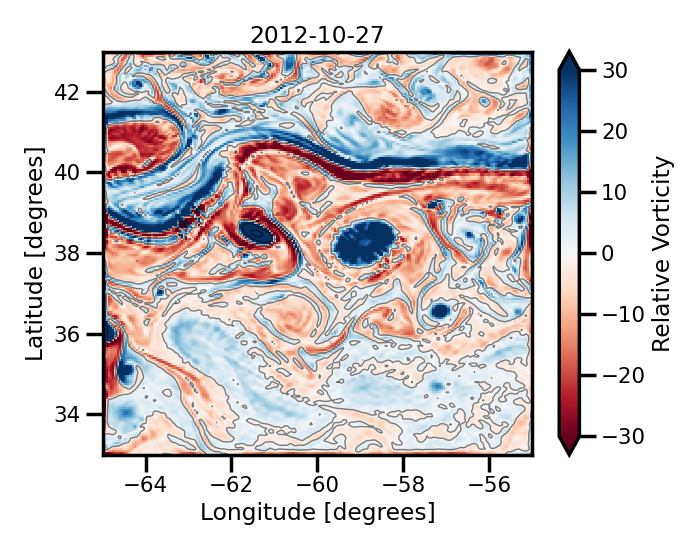
\includegraphics[trim={0 0 42mm 0},clip, width=3.20cm,height=3cm]{content/figures/maps/rvort/dc20a/nadir4/dc20a_nemo_vort_r.png} &
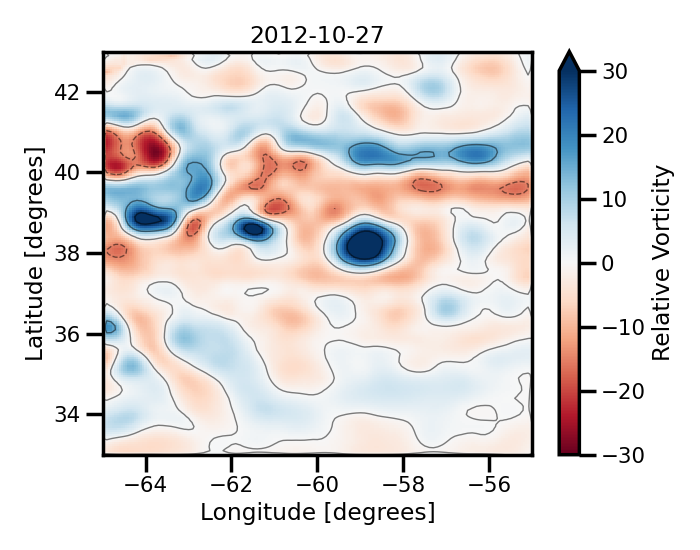
\includegraphics[trim={0 0 42mm 0},clip, width=3.2cm,height=3cm]{content/figures/maps/rvort/dc20a/nadir4/dc20a_miost_vort_r.png} &
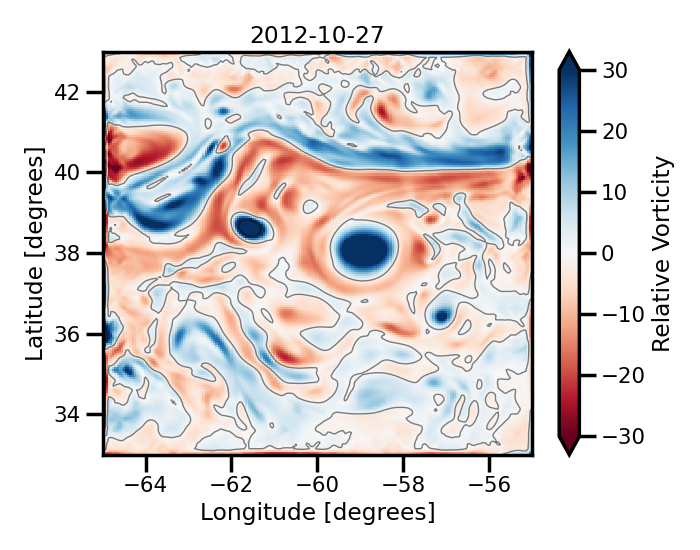
\includegraphics[trim={0 0 42mm 0},clip, width=3.2cm,height=3cm]{content/figures/maps/rvort/dc20a/nadir4/dc20a_bfnqg_vort_r.png} &
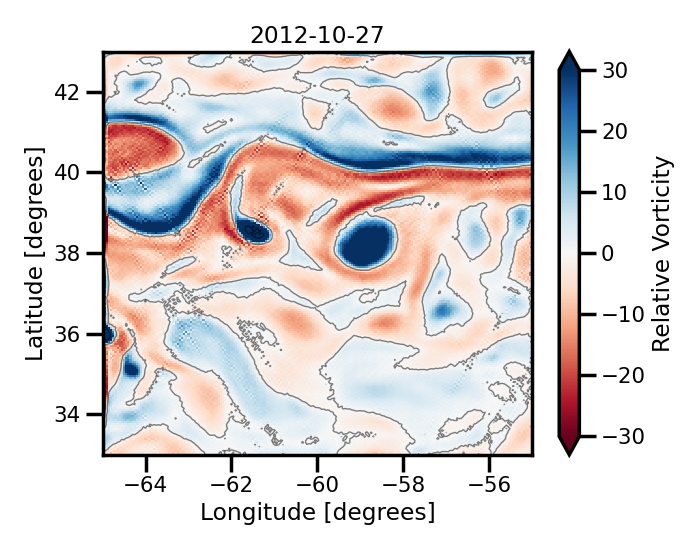
\includegraphics[width=4.0cm,height=3cm]{content/figures/maps/rvort/dc20a/nadir4/dc20a_4dvarnet_vort_r.png}  \\
%%%%% STRAIN %%%%%%%%
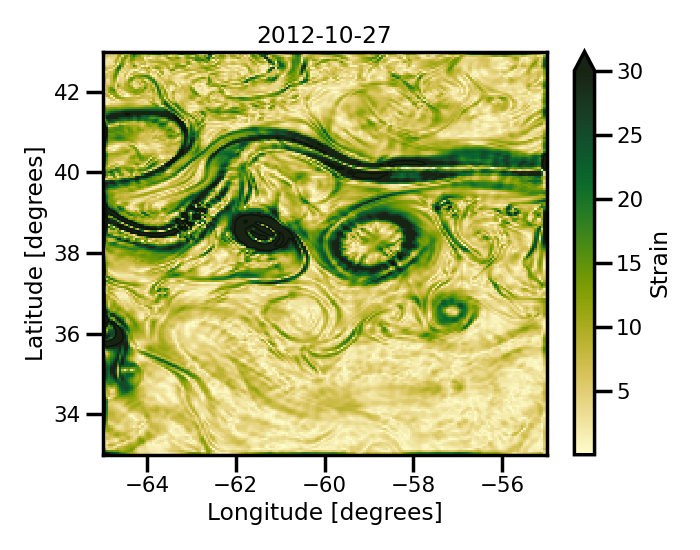
\includegraphics[trim={0 0 38mm 0},clip, width=3.20cm,height=3cm]{content/figures/maps/strain/dc20a/nadir4/dc20a_nemo_strain.png} &
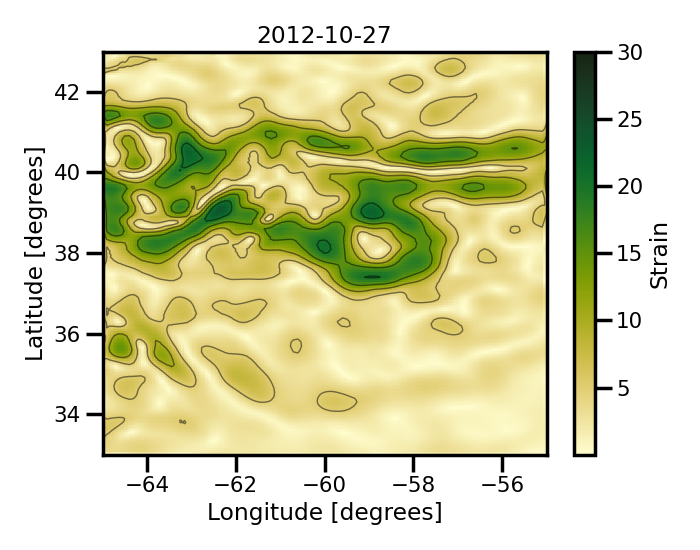
\includegraphics[trim={0 0 38mm 0},clip, width=3.2cm,height=3cm]{content/figures/maps/strain/dc20a/nadir4/dc20a_miost_strain.png} &
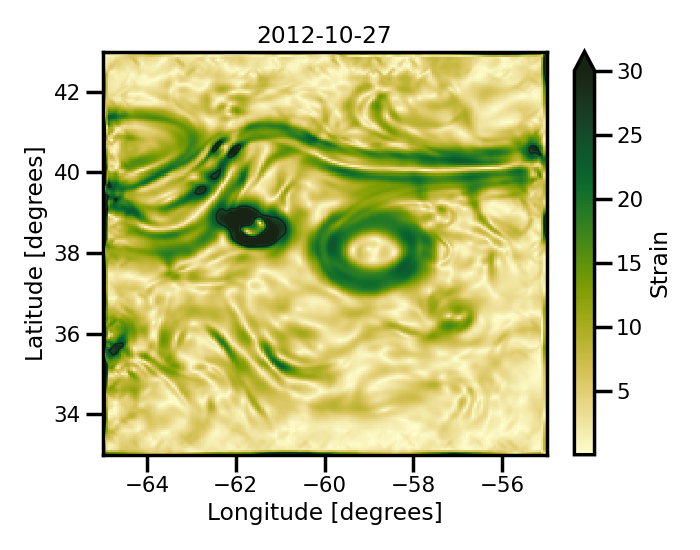
\includegraphics[trim={0 0 38mm 0},clip, width=3.2cm,height=3cm]{content/figures/maps/strain/dc20a/nadir4/dc20a_bfnqg_strain.png} &
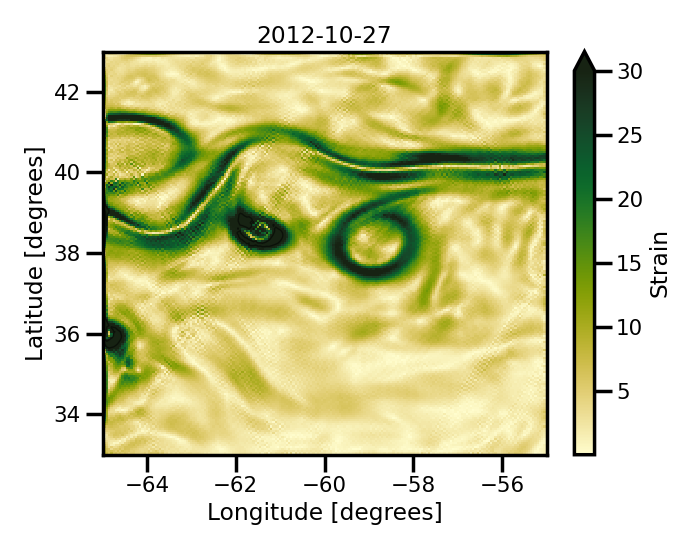
\includegraphics[width=4.0cm,height=3cm]{content/figures/maps/strain/dc20a/nadir4/dc20a_4dvarnet_strain.png}  \\
% \vspace{-2mm}
(a) & (b) & (c) & (d)
\end{tabular}
\vspace{-3mm}
% \caption{Row I - Isotrophic PSD. Row 2 - Isotrophic PSD Score}
\caption{
A snapshot at $27^{th}$ October, 2012 of the sea level anomaly (SLA) from the NEMO simulation for the OSSE experiment outlined in section~\ref{sec:experimental_design}. 
The top row showcases the aggregated NADIR altimetry tracks and the aggregated SWOT altimetry tracks (12 hours before and 12 hours after) as well as the SST from the NEMO simulation.
Each subsequent row showcases the following physical variables found in appendix~\ref{sec:physical_variables}: (a) Sea Level Anomaly, (b) Kinetic Energy, (c) Relative Vorticity, and (d) Strain. 
Each column in the subsequent rows showcase the following reconstructed field from the NEMO simulation found in columrn (a): (b) MIOST~\cite{MIOST}, (c) BFN-QG~\cite{BFNQG}, and (d) 4DVarNet~\cite{4DVARNETSWOT}.}
\vspace{-5mm}
\label{fig:oceanbench_maps}
\end{center}
\end{figure}


% \subsubsection{Observing System Experiments (OSE)} \label{sec:ose}

\textbf{Observing System Experiments (OSE)}. As more observations have become available over the past few decades, we can also design experiments using real data. 
This involves aggregating as many observations from real ocean altimetry satellites as possible with some specific independent subset left out for evaluation purposes.
A major downside to OSE experiments is that the sparsity and spatial coverage of the observations narrow the possible scope of performance metrics and make it very challenging to learn directly from observation datasets. 
The current standard altimetry data are high resolution but cover a tiny area. 
As such, it can only inform fine-scale SSH patterns in the along-track satellite direction and cannot explicitly reveal two-dimensional patterns. 
Despite these drawbacks, it provides a quantitative evaluation of the generalizability of the ML methods concerning the true ocean state.
%and so it fails to capture many of the dynamical regimes we are interested in, i.e. mesoscale and sub-mesoscale processes. 
%However, it is still advantageous (and preferable) to include these experiments because these reflect the true ocean state and will help with the generalizability of the ML methods.

\begin{figure}[t!]
\small
\begin{center}
\setlength{\tabcolsep}{2pt}
\begin{tabular}{ccc}
% $\mathcal X$ & $\hat \z = \bG_\theta(\x)$ & $\x = \bG_\theta^{-1} (\hat \z)$\\[0mm]
% NATL60&
% \multicolumn{2}{c}{\includegraphics[width=6.25cm,height=4.5cm]{content/figures/exp_natl60/psd_st/osse_2020a_psd_natl60}} 
% \\
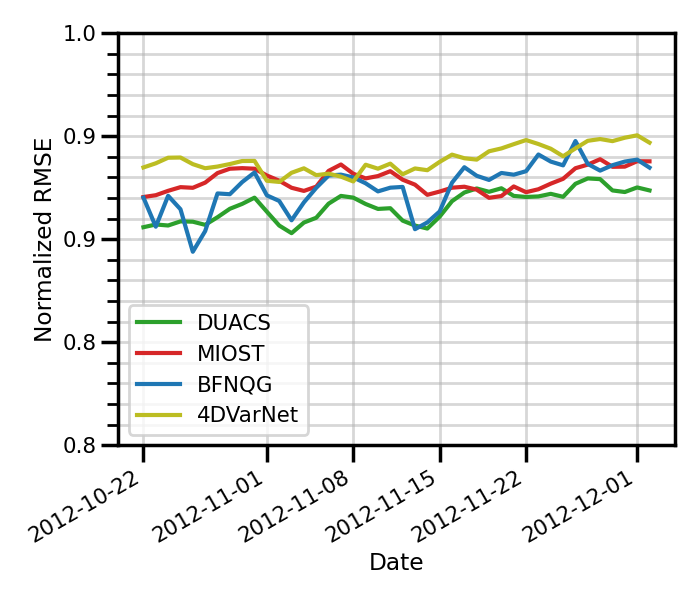
\includegraphics[width=3.75cm,height=3.25cm]{content/figures/stats/nrmse_space.png} &
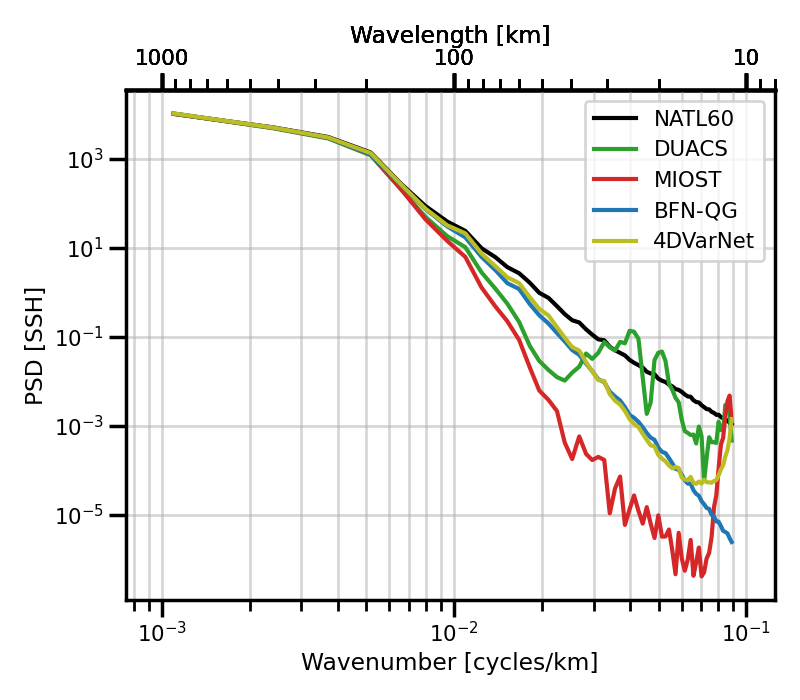
\includegraphics[width=4.25cm,height=3.5cm]{content/figures/psd_isotropic/dc20a/nadir4/dc20a_psd_iso_ssh.png} &
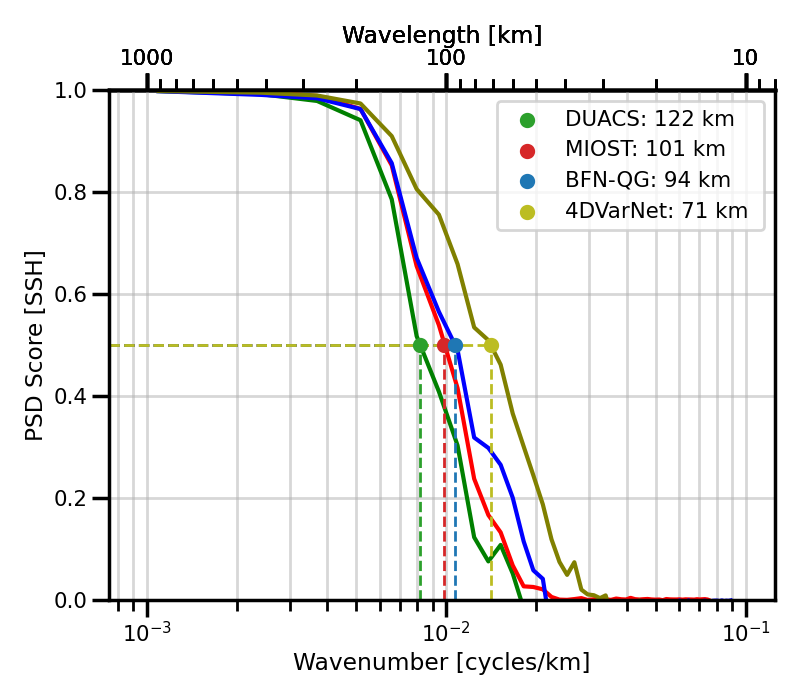
\includegraphics[width=4.25cm,height=3.5cm]{content/figures/psd_isotropic/dc20a/nadir4/dc20a_psd_score_iso_ssh.png} 
\\
(a) Normalized RMSE &
(b) Isotropic Power Spectrum &
(c) Isotropic Power Spectrum Score
\end{tabular}
\begin{tabular}{cccc}
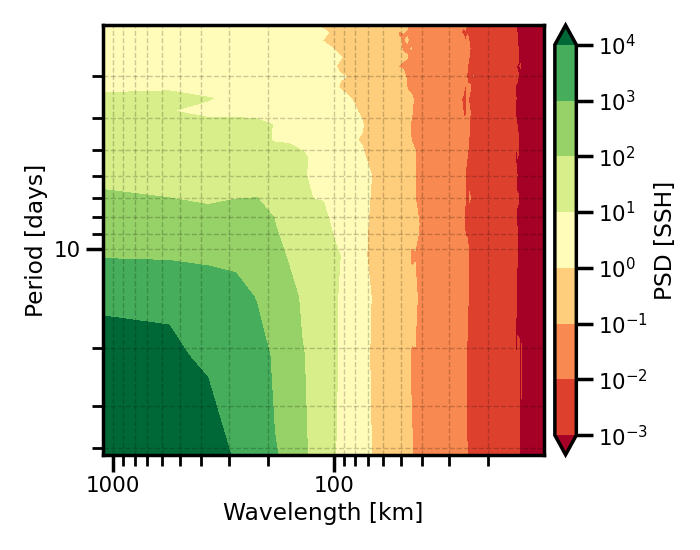
\includegraphics[trim={0 0 0mm 0},clip, width=4.20cm,height=3cm]{content/figures/psd_spacetime/dc20a/nadir4/dc20a_psd_spacetime_nemo_nadir4_ssh.png}  &
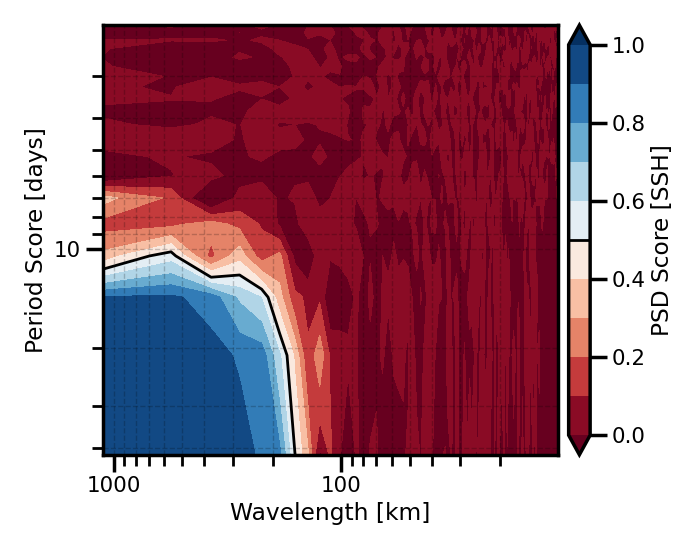
\includegraphics[trim={20mm 0 34mm 0},clip, width=2.9cm,height=3cm]{content/figures/psd_spacetime/dc20a/nadir4/dc20a_psd_spacetime_score_miost_nadir4_ssh.png} &
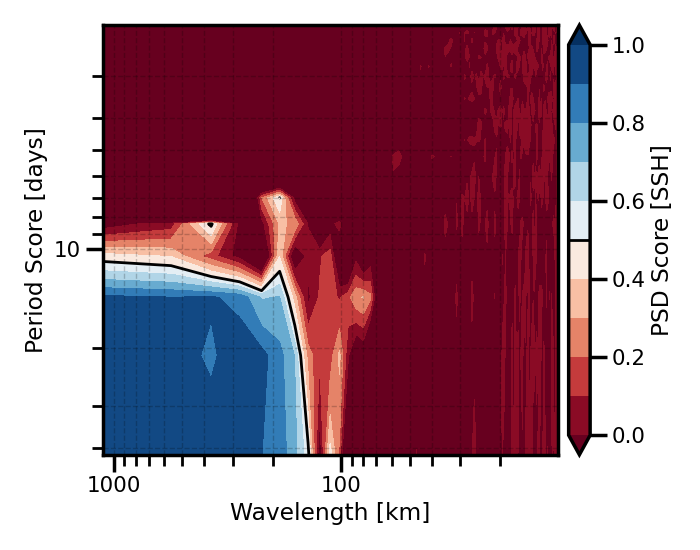
\includegraphics[trim={20mm 0 34mm 0},clip, width=2.9cm,height=3cm]{content/figures/psd_spacetime/dc20a/nadir4/dc20a_psd_spacetime_score_bfnqg_nadir4_ssh.png} &
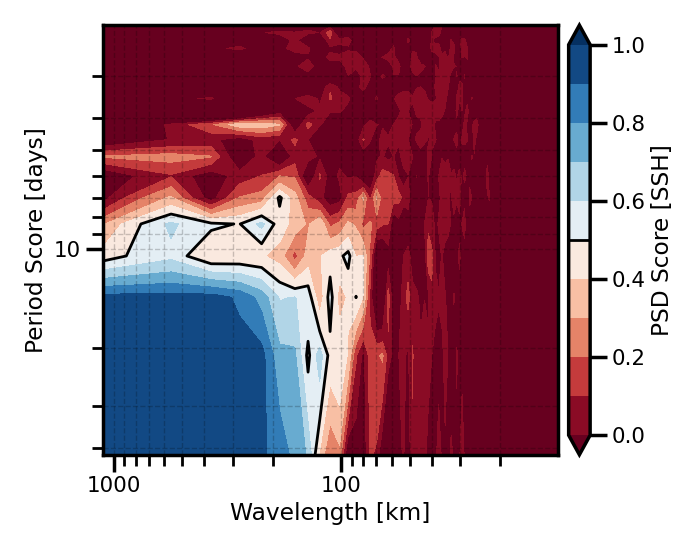
\includegraphics[trim={20mm 0 0 0},clip, width=3.5cm,height=3cm]{content/figures/psd_spacetime/dc20a/nadir4/dc20a_psd_spacetime_score_4dvarnet_nadir4_ssh.png} \\
(d) NEMO Simulation &
(e) MIOST &
(f) BFN-QG &
(g) 4DVarNet
\end{tabular}
% % \vspace{-4mm}
% \caption{Row I - Isotrophic PSD. Row 2 - Isotrophic PSD Score}
\caption{This figure showcases some statistics for evaluation of the SSH field reconstructions for the OSSE NADIR experiment outlined in section~\ref{sec:interp_challenge}. Subfigure (a) showcases the normalized root mean squared error (nRMSE), (b) showcases the isotropic power spectrum decomposition (PSD), (c) showcases isotropic PSD scores.
The bottom row showcases the space-time power spectrum decomposition (PSD) for the NEMO simulation (subfigure (d)) and the PSD scores for three reconstruction models: (e) the MIOST model~\cite{MIOST}, (f) the BFN-QG model~\cite{BFNQG}, and (g) the 4DVarNet model~\cite{4DVARNETSWOT}.
}
% \vspace{-5mm}
\label{fig:oceanbench_psd}
\end{center}
\end{figure}


%
\subsection{Data Challenges} \label{sec:data_challenges}

We rely on existing OSSE and OSE experiments for SSH interpolation designed by domain experts~\cite{DCOSEGULFSSH,DCOSSEGULFSSH} and recast them into \texttt{OceanBench} framework to deliver a ML-ready benchmarking suites. 
The selected data challenges  for this first edition address SSH interpolation for a 1000km$\times$1000km Gulfstream region. We briefly outline them below.
%The \textit{Ocean-Data-Challenge} group has a wide-range of different OSSE and OSE experiments involving SSH interpolation in particular~\cite{DCOSEGULFSSH,DCOSSEGULFSSH}. 
%For this paper, we will focus on a subset and demonstrate some evaluation steps generated from the \texttt{OceanBench} framework.
%We outline an experimental setup SSH reconstruction over the Gulfstream with three OSSE's configurations and one OSE configuration in the next section. For more detailed information about the experimental setups for each configuration, see section~\ref{sec:data_challenges_extended} in the appendix.

% \begin{itemize}
%     \item 
\textbf{Experiment I (\textit{OSSE NADIR})} addresses SSH interpolation using NADIR altimetry tracks which are very fine, thin ocean satellite observations (see Figure~\ref{fig:oceanbench_maps}). It relies on an OSSE using high-resolution ($1/60^\circ$ resolution) ocean simulations generated by the NEMO model over one year with a whole field every day. 

%The observation data uses NADIR altimetry tracks which are very fine, thin ocean satellite observations (see Figure~\ref{fig:oceanbench_maps} (a) \& (b)). 
\textbf{Experiment II (\textit{OSSE SWOT})} addresses SSH interpolation using jointly NADIR and SWOT altimetry data where we complement the \textbf{OSSE NADIR} configuration with simulated SWOT observations.
SWOT is a new satellite altimetry mission with a much higher spatial coverage but a much lower temporal resolution as illustrated in Figure~\ref{fig:oceanbench_maps}.
The higher spatial resolution allows us to see structures at a smaller resolution but at the cost of a massive influx of observations (over $\times$100).

\textbf{Experiment III (\textit{OSSE SST})} addresses SSH interpolation using altimetry and SST satellite data jointly. We complement the \textbf{OSSE SWOT} challenge with simulated SST observations. 
Satellite-derived SST observations are more abundantly available in natural operational settings than SSH at a finer resolution, and structures have visible similarities~\cite{SWOT,BFNQG}.
So this challenge allows for methods to take advantage of multi-modal learning~\cite{4DVARNETSST,SSHInterpAttention}.

\textbf{Experiment IV (\textit{OSE NADIR})} addresses SSH interpolation for real NADIR altimetry data. 
In contrast to the three OSSE data challenges, it only looks at actual observations aggregated from the currently available ocean altimetry data from actual satellites. 
It involves a similar space-time sampling as Experiment (\textbf{OSSE NADIR}) to evaluate the generalization of ML methods trained in Experiment I to real altimetry data. 
The training problem's complexity increases significantly due to the reference dataset's sparsity compared with the \textbf{OSSE NADIR} dataset. 
One may also explore transfer learning or fine-tuning strategies from the available OSSE dataset. 


% \begin{itemize}
%     \item Experiment I (\textbf{OSSE NADIR}) addresses SSH interpolation using NADIR altimetry tracks which are very fine, thin ocean satellite observations (see Figure~\ref{fig:oceanbench_maps}). It relies on an OSSE using anocean simulations generated by the NEMO model, more precisely a high-resolution simulation, $1/60^\circ$ resolution, over one year with a whole field every day. 
% %The observation data uses NADIR altimetry tracks which are very fine, thin ocean satellite observations (see Figure~\ref{fig:oceanbench_maps} (a) \& (b)). 
% \item Experiment II (\textbf{OSSE SWOT}) addresses SSH interpolation using jointly NADIR and SWOT altimetry data. We complement the \textbf{OSSE NADIR} configuration with simulated SWOT observations.  
% SWOT is a new satellite altimetry mission with  much higher spatial coverage but a much lower temporal resolution as illustrated in Figure~\ref{fig:oceanbench_maps}.
% The higher spatial resolution allows us to see structures at a smaller resolution but at the cost of a massive influx of observations (over $\times 100$).
% \item Experiment III (\textbf{OSSE SST}) addresses SSH interpolation using 
% jointly altimetry and SST satellite data. We complement the \textbf{OSSE SWOT} challenge with simulated SST observations. 
% Satellite-derived SST observations are more abundantly available in natural operational settings than SSH at a finer resolution, and structures have visible similarities \cite{}.
% So this challenge allows for methods to take advantage of multi-modal learning \cite{}.
% \item Experiment IV \textbf{OSE NADIR} addresses SSH interpolation for real NADIR altimetry data. In contrast to the three OSSE data challenges, it only looks at actual observations aggregated from the currently available ocean altimetry data from actual satellites. It involves a similar space-time sampling as Experiment (\textbf{OSSE NADIR}) to evaluate the generalization of ML methods trained in Experiment I to real altimetry data. Besides, one may also explore learning or fine-tuning strategies from the available OSE dataset. We may point out that the complexity of the training problem due to the sparsity of refence dataset compared with \textbf{OSSE NADIR} dataset.
% \end{itemize}




\subsection{\texttt{OceanBench} Pipelines}

For the four data challenges presented in the previous section, we implemented \texttt{OceanBench} pipelines to deliver a ML-ready benchmarking framework.
We used the \texttt{hydra} and the geoprocessing tools outlined in section~\ref{sec:code_structure} with specialized routines for regridding the ocean satellite data to a uniformly gridded product and vice versa when necessary. 
Appendix~\ref{sec:hydra_recipes} showcases an example of the hydra integration for the preprocessing pipeline. 
A key feature is the creation of a custom patcher for the appropriate geophysical variables using our \texttt{XRPatcher} tool, which is later integrated into custom datasets and dataloaders for the appropriate model architecture, e.g., coordinate-based or grid-based. 
We provide an example snippet of how this can be done easily in section~\ref{sec:xrpatcher}.
\texttt{OceanBench} also features some tools specific to the analysis of SSH. 
For example, physically-interpretable variables like geostrophic currents and relative vorticity, which can be derived from first-order and second-order derivatives of the SSH, are essential for assessing the quality of the reconstructions generated by the models. 
Figure~\ref{fig:oceanbench_maps} showcases some fields of the most common physical variables used in the oceanography literature for the SSH-based analysis of sea surface dynamics. For more details regarding the nature of the physical variables, see appendix~\ref{sec:physical_variables}.

Regarding the evaluation framework, we include domain-relevant performance metrics beyond the standard ML loss and accuracy functions. They account for the sampling patterns of the evaluation data. Spectral analytics are widely used in geoscience~\cite{BFNQG}, and here, we consider spectral scores computed as the minimum spatial and temporal scales resolved by the reconstruction methods proposed in~\cite{BFNQG}.
For example, figure~\ref{fig:oceanbench_psd} showcases how \texttt{OceanBench} generated the isotropic power spectrum and score and the space-time power spectrum decomposition and score.
Table~\ref{tb:oceanbench_results} outlines some standard and domain-specific scores for the experiments outlined in section~\ref{sec:experimental_design}.
We give a more detailed description of the rationale and construction of the power-spectrum-specific metrics in appendix~\ref{sec:metrics}. In terms of baselines, we report for each data challenge the performance of at least one approach for each of the category outlined in Section \ref{sec:ml_ontology_mini}.


\begin{table}[h]
\caption{This table highlights some of the results for the \textbf{OSSE NADIR} experiment outlined in section~\ref{sec:data_challenges} and appendix~\ref{sec:data_challenges_extended}.
% and the OSE experiment outlined in section~\ref{sec:ose}~\tocite{}. 
% For more results regarding the SWOT data, please see section~\ref{sec:other_tasks}. 
This table highlights the performance statistically in the real and spectral space; the normalized RMSE for the real space and the minimum spatial and temporal scales resolved in the spectral domain. 
For more information about the class of models displayed and class of metrics, see appendix~\ref{sec:ml_ontology} and appendix~\ref{sec:metrics} respectively. We only showcase the model performance on the alongtrack NADIR data available. For the extended table for each of the challenges, see Table~\ref{tb:exp-results-mega}.}
\label{tb:oceanbench_results}
\centering
\begin{tabular}{lllcccc}
 \toprule
% Experiment & Configuration & Method & nRMSE & Resolved Scale [km]    \\ \midrule
% \multirow{2}{*}{Experiment} & \multirow{2}{*}{Algorithm} & \multirow{2}{*}{Algorithm Class} & \multirow{2}{*}{nRMSE} & \multicolumn{2}{c}{Effective Resolution} \\ 
% &  &   &  & Wavelength [km]  & Period [days]      \\ \midrule
% \multirow{2}{*}{Experiment} & \multirow{2}{*}{Algorithm} & \multirow{2}{*}{Algorithm Class} & \multirow{2}{*}{nRMSE} & \multicolumn{2}{c}{Effective Resolution} \\ 
Experiment &  Algorithm &   Algorithm Class &  nRMSE & $\lambda_{\mathbf{x}}$ [km]  & $\lambda_{t}$ [days]      \\ \midrule
\multicolumn{1}{l}{OSSE NADIR}     &  OI~\cite{DUACS} &  Coordinate-Based & 0.92 $\pm$ 0.01 & 175 & 10.8 \\
\multicolumn{1}{l}{OSSE NADIR}     &  MIOST~\cite{MIOST} &  Coordinate-Based  & 0.93 $\pm$ 0.01 & 157 & 10.1 \\
\multicolumn{1}{l}{OSSE NADIR}     &  BFNQG~\cite{BFNQG} &  Hybrid Model   & 0.93 $\pm$ 0.01 & 139 & 10.6 \\
OSSE NADIR &  4DVarNet~\cite{4DVARNETSWOT} &  Bi-Level Opt.  & 0.95 $\pm$ 0.01 & 117 & 7.7 \\
\bottomrule
\end{tabular}
\end{table}

